% !TEX root = ../Thesis.tex

\chapter{Background}
Before we dive into how we can translate Sudokus into a language such that a computer can work on them, we first elaborate on some background knowledge and definitions needed to understand the used tools and formalisms.

\section{Propositional Logic}
Propositional logic is a language that provides a formal way of writing statements that can either be true or false. It is used in this thesis to describe and encode the specific rules of the different Sudoku Variants. This section will shortly introduce the common syntax and semantics.

\paragraph{Atoms}
(also called \emph{atomic propositions}) are the smallest units used in propositional logic, and must have a truth value of true or false (often noted as digits 0 and 1).

\paragraph{Literals}
are atoms or their negation, so if $x_1$ is an atom, then $x_1$ and $\neg x_1$ are literals. Literals are said to be \emph{positive} or \emph{negative} respectively.


\paragraph{Formulas} are compositions of one or multiple atoms and can be defined recursively:\\
Every atom is also a formula.
If $\varphi$ is a formula, then so is its negation $\neg\varphi$.
If $\varphi$ and $\psi$ are formulas, then so is the conjunction $\varphi \land \psi$.
If $\varphi$ and $\psi$ are formulas, then so is the disjunction $\varphi \lor \psi$.


\paragraph{Interpretations} (also called truth assignments) are functions that assigns truth values to a set $A$ of atoms $\mathcal{I}: A \rightarrow \{0,1\}$. A formula $\varphi$ over $A$ holds (is true) under an interpretation $\mathcal{I}$ (written $\mathcal{I} \models \varphi$) following the semantical rules:
\begin{center}
    \begin{tabular}{ l l l }
    $\mathcal{I} \models x_1$ & iff & $\mathcal{I}(x_1) = 1$\\
    $\mathcal{I} \models \neg x_1$ & iff & not $\mathcal{I} \models x_1$\\
    $\mathcal{I} \models (\psi \land \varrho)$ & iff & $\mathcal{I} \models \psi$ and $\mathcal{I} \models \varrho$\\
    $\mathcal{I} \models (\psi \lor \varrho)$ & iff & $\mathcal{I} \models \psi$ or $\mathcal{I} \models \varrho$\\
\end{tabular}\\
Where $\psi$ and  $\varrho$ are formulas and $x_1$ is an atom.
\end{center}An interpretation for which a formula $\varphi$ hold is called a \emph{model} of $\varphi$.

\paragraph{Equivalence}
of two formulas $\varphi$ and $\psi$ is given if it holds for all interpretations $\mathcal{I}$ that, $\varphi$ holds under $\mathcal{I}$ if and only if $\psi$ holds under $\mathcal{I}$. The formulas are then called \emph {logically equivalent} ($\varphi \equiv \psi$).

\paragraph{Implications / Biconditionals}
As one might have noticed, implication ($\rightarrow$) and biconditional ($\leftrightarrow$) have not been mentioned in the definition of formulas as they are abbreviations for more extended formulas that use $\lor$, $\land$ and $\neg$.
\begin{center}
\begin{tabular}{ l l l }
    $(\varphi \rightarrow \psi)$ & $\equiv$ & $(\neg\varphi \lor \psi)$\\
    $(\varphi \leftrightarrow \psi)$ & $\equiv$ & $(\neg\varphi \lor \psi) \land (\neg\psi \lor \varphi)$\\
\end{tabular}
\end{center}

\paragraph{Clauses}
are disjunctions of literals (atoms and/or their negations). A formula that is a clause is true under interpretation $\mathcal{I}$ if one of its literals is true.

\paragraph{Conjunctive Normal Form (CNF)}
A formula is said to be in conjunctive normal form if it is a conjunction of clauses. 
For example, given the atoms \emph{a}, \emph{b}, \emph{c} and \emph{d}, the formulas $\varphi$, $\psi$ and $\varrho$ are in CNF:
\begin{center}
    \begin{tabular}{ l l l }
    $\varphi$ & $\equiv$ & $(a)$\\
    $\psi$ & $\equiv$ & $(a \land b)$\\
    $\varrho$ & $\equiv$ & $((a \lor b) \land (c \lor d))$\\
\end{tabular}
\end{center}
Also, it holds that every formula can be brought into CNF \cite{LogicForComputerScientists}, and a formula in CNF can be noted as a set of sets of literals, for example, $\varrho \equiv \{\{a,b\},\{c,d\}\}$.

\section{SAT-Problems and SAT-Solvers}
SAT-Problems (also called \emph{Satisfiability Problems} or \emph{Boolean Satisfiability Problems}) describe the problem of deciding if a formula of propositional logic is satisfiable (if there exists a model for it) or not. SAT-solvers are programs or algorithms that try to solve instances of this problem. They take a formula as input and return a boolean value (true or false) to indicate if a model exists or not. Most SAT-solvers also directly provide a model if they can find one. In the experiments of this thesis, multiple SAT-solvers are used, which are described in further detail in \ref{MiniSatAndSat4j}. As we will later see, the time to find solutions for particular problem instances varies between them. However, when it comes to computational complexity, it holds that SAT-Problems are in NP and that they are NP-Hard\cite{10.1145/800157.805047}\cite{levin1973universal}, so the runtime of the solvers may scale exponentially with the number of clauses and variables given to them as input.

\subsection{DIMACS CNF File Format}\label{DIMACS}
The used SAT-solvers require the input formula to be in CNF. Further, they expect them to be described in the DIMACS CNF File Format, often just called DIMACS. The abbreviation DIMACS stands for Center for ``Discrete Mathematics and Theoretical Computer Science", which is a collaboration between Rutgers and Princeton University and research firms. The file format was utilised in the DIMACS Implementation Challenge 1993 and since then has become the common file format for SAT-Problems.\\

DIMACS CNF Files have the following Format:
\begin{itemize}
    \item Atoms are represented as positive integers.
    \item Negative literals are represented as negative integers.
    \item The first line starts with the letter ``p" and holds the problem description. It states the problem type, the highest integer used to describe an atom and the number of clauses.
    \item Clauses are represented as lists of their literals and are terminated by the number 0. White spaces or line breaks separate all literals and the ending 0s.
    \item Lines are interpreted as comments (ignored by the solver) if they start with the letter ``c". Comments can be added everywhere in the file except inside the definition of a clause.
\end{itemize}
A DIMACS file describing the formula $\varphi \equiv (x_1 \lor \neg x_2) \land (x_2 \lor x_3) \land (\neg x_1 \lor \neg x_3) \land (\neg x_1 \lor \neg x_2 \lor x_3)$ could look like this:

\lstset{basicstyle=\ttfamily}
\begin{lstlisting}[language=Java,frame=single]
c some comment describing the problem
p cnf 3 4
 1 -2  0
 2  3  0
-1 -3  0
-1 -2  3  0
\end{lstlisting}


\subsection{How SAT-Solvers solve}
Given a formula, a SAT-solver must decide if it is satisfiable or not (We assume the formula is in CNF so it can be handled as a set of clauses). To do so, the solver tries to find a model by assigning truth values to atoms one by one. In a standard SAT-solver, this is not done randomly but by using the inference mechanism of \emph{unit propagation}. 
A famous algorithm using this mechanism is the DPLL algorithm \cite{DavisAMachineProgramForTheoremProving1962} which can be directly implemented into a SAT-solver.
DPLL applies three rules:
\begin{enumerate}
    \item If a clause contains only one literal (or multiple literals, but only one is still unbound and all the others do not make the clause true),  the value that makes the literal true must be assigned. Otherwise, the clause and the formula would become false. If a value gets assigned, all clauses containing the corresponding true literal can be removed from the set of clauses. The corresponding false literals can be removed from all remaining clauses since they can not make them true.
    \item If there is a literal that only appears in one polarity in all clauses (consistently positive/negative), its atom value can also be assigned to make the literals true.
    \item  If the set of clauses becomes empty, the formula is ``satisfiable". If an empty clause is derived, the formula is ``unsatisfiable". If no further assignments can be inferred and no decision can be made about satisfiability yet, a literal gets chosen. The algorithm would then continue in two branches, one where the chosen literal gets set to be true and one where it is set to be false. The formula is then satisfiable if and only if it is satisfiable under one of the two assumptions. Repeating this procedure of assigning values creates a Search-Tree of exponential size.
\end{enumerate}
SAT-solvers can strongly differentiate in how they choose the next atom to assign a value to and how they learn from entering unsatisfiable branches in the search tree.



\subsection{MiniSat and Sat4j}\label{MiniSatAndSat4j}
MiniSat is a lightweight SAT-solver that is based on ``the ideas for conflict-driven backtracking, together with watched literals and dynamic variable ordering" as the original paper \cite{EenAnExtensibleSAT-solver2004} states. Its original source code in C++ used less than 600 lines. The solver was further refined up to its current version 2.2, but for the experiments in this thesis we use version 1.4 for which precompiled binaries can be found at \cite{webMiniSat}.

Sat4j is a Java library that provides a SAT-solver that can be directly called and run in Java. It does not provide the best performance, but because it is easy to use and integrate, it is well suited for early experimenting and testing. The used version is 2.3.4. The library itself and further details can be found at \cite{webSat4j}.

MiniSat+ (a particular version of MiniSat) and Sat4j provide native support for Pseudo-Boolean Constraints. However, this feature will not be used because this thesis aims to translate Sudoku Puzzles into a form that can be solved with arbitrary SAT-solvers.

\section{Constraint Networks (CN)}
Puzzles like Sudoku can be broken down into multiple constraints that must all hold for a solution to be correct. Problems like this can be described using constraint networks. The issue of finding a solution to a constraint network is called Constraint Satisfaction Problem or short CSP. Solutions for constraint networks can be found using Backtracking Search (\cite{ArtificialAModernApproach}, page 175).However, this thesis aims to find such solutions by first encoding the Constraints into SAT-Problems that arbitrary SAT-solvers can then solve. This section will shortly discuss how constraint networks are defined and how they can be translated directly to general SAT-Problems.


Constraint Networks can be described as a tuple of three components: $CN := \langle \mathcal{X},  \mathcal{D},  \mathcal{C}\rangle$.
$\mathcal{X}$ is a set of variables, $\mathcal{D}$ is a set of finite domains (one corresponding to each variable), and $\mathcal{C}$ is a set of constraints that describe the allowed values for variable subsets.

\subsection{Unary Constraints}
Constraints that only consider one variable are called unary constraints. They do not have to be explicitly written as part of $\mathcal{C}$ because they can also be seen as a domain restriction for a variable that can be represented by reducing the corresponding domain. Examples for a variable $x_1$ could be: ``$x_1$ must be smaller than 10", ``$x_1$ must be larger than 0", or ``$x_1$ must be even".

\subsection{Binary Constraints}
Constraints that include two variables are called binary constraints. They get defined extensively as part of $\mathcal{C}$ by listing all allowed value pairs that the two variables could take. Examples for CSP variables $x_1$ and $x_2$ could be: ``$x_1$ must be smaller than $x_2$", ``$x_1$ or $x_2$ must be 9", or ``$x_1 + x_2 \leq 12$".

\subsection{N-ary Constraints}
Constraints that include more than two variables are called N-nary constraints and get defined similarly to binary constraints in a CSP. Examples for variables $x_1$ to $x_9$ could be: ``At most one CSP variable from $x_1$ to $x_9$ may be 5" or ``The sum of the CSP variables $x_1$ to $x_9$ must be 45".

\subsection{Common Encodings}
There are many different ways to transform a CSP into a set of clauses that a SAT-solver can work on, two of the most common ones we want to elaborate on here.

\paragraph{Direct Encoding \cite{walsh2000SATvCSP}\cite{gent20002ArcConsistencyInSAT}}
We assign a SAT variable $x_{i,j}$ to all possible variable values $j$ for all CSP variables $i$. \emph{At-least-one} clauses ensure that a CSP variable i has at least one out of the $d$ values assigned from its domain.
\begin{center}
    $x_{i,1} \lor x_{i,2} \lor ... \lor x_{i,d}$
\end{center}

\emph{At-most-one} clauses ensure that a CSP variable $i$ has at most one value assigned from its domain.
\begin{center}
    $\neg x_{i,j} \lor \neg x_{i,k}$\\
    $\forall x_{i,j}, x_{i,k} \in D_i$ s.t. $j\neq k$ 
\end{center}

\emph{Conflict} clauses ensure that no CSP variable value combinations are allowed that do not comply with the CSP's constraints.
For example, The N-ary constraint ``at most one CSP variable of $x_1$, $x_2$ and $x_3$ has value 5" would be transformed into the following conjunction of clauses:
\begin{center}
 $(\neg x_{1,5} \lor \neg x_{2,5}) \land (\neg x_{1,5} \lor \neg x_{3,5}) \land (\neg x_{2,5} \lor \neg x_{3,5})$. 
\end{center}

Assuming the CSP has $n$ variables that have a domain of size $d_i$, the transformation would in total lead to $n$ at-least-one clauses and per variable to $\sum_{m=1}^{d_i} (m-1)$ at-most-one clauses. For the constraints, however, we can only give an upper bound for the number of needed clauses per constraint equal to the product of the domain sizes of the contained variables.

\paragraph{Support Encoding \cite{kasif1990OnTheParallelComplexityOfDiscreteRelaxationInConstraintSatisfactionNetworks}\cite{gent20002ArcConsistencyInSAT}}
The same at-least-one and at-most-one clauses are used as in the direct encoding, but instead of conflict clauses, we add so-called support clauses. For all pairs of variables $x_i$ and $x_j$ in a constraint, we add a clause for all domain values of $x_j$. These clauses define the allowed values of the other variables of the constraint.However, not all these clauses must be necessary. They can be left away if the CSP variable value corresponding to $x_{j,d}$ is allowed with all values of CSP variable $x_i$. 
This is best shown in an example, assume all CSP variables have a domain of \{1, 2, 3, 4, 5\}, the N-ary constraint ``at most one CSP variable of $x_1$, $x_2$ and $x_3$ has value 5” could then be transformed to the clauses:
\begin{center}
 $\neg x_{1,5} \lor x_{2,1} \lor x_{2,2} \lor x_{2,3} \lor x_{2,4}$\\
 $\neg x_{2,5} \lor x_{1,1} \lor x_{1,2} \lor x_{1,3} \lor x_{1,4}$\\
 $\neg x_{1,5} \lor x_{3,1} \lor x_{3,2} \lor x_{3,3} \lor x_{3,4}$\\
 $\neg x_{3,5} \lor x_{1,1} \lor x_{1,2} \lor x_{1,3} \lor x_{1,4}$\\
 $\neg x_{2,5} \lor x_{3,1} \lor x_{3,2} \lor x_{3,3} \lor x_{3,4}$\\
 $\neg x_{3,5} \lor x_{2,1} \lor x_{2,2} \lor x_{2,3} \lor x_{2,4}$\\
\end{center}
In this case further clauses like $\neg x_{1,1} \lor x_{2,1} \lor x_{2,2} \lor x_{2,3} \lor x_{2,4} \lor x_{2,5}$ can be added, but they are redundant because if the CSP variable $x_1$ takes the value 1 the constraint does allow all possible values for $x_2$. Generally, the support encoding requires more clauses than the direct encoding, but this does not make it inferior or necessarily slower for SAT-solvers \cite{gent20002ArcConsistencyInSAT}. 


\subsection{Pseudo-Boolean Constraints (PBCs)}
Constraints that describe equations like $w_1x_1+w_2x_2+...+w_nx_n \leq K$ are called Pseudo-Boolean Constraints. The variables $x_1$ to $x_n$ have boolean domains, the $w_i$s are called weights, and K is called bound (or RHS). Both the weights and the bound must have integer values. If a variable $x_i$ gets assigned a truth value of true/false, it gets valued 1/0 in the equation. PBCs can be transformed into clauses by first converting them to Binary Decision Diagrams (BDD), Adder Networks or Sorter Networks. Within this thesis, we will use the former two variants following the ideas of \cite{Een2006TranslatingPC}, which we will elaborate on further in section \ref{encoding:PBCs}.

\section{Sudoku}\label{NormalSudoku}
The family of logic puzzles called Sudoku is based on the Latin Squares Problem. In its current form, it was first published in the US in 1979 by Howard Garns as ``Number Place". In 1984 the puzzle became popular in Japan,  where it got the name ``Sudoku" (translated: ``digit-single") which is the name under which it later became famous around the world.
A \emph{normal} Sudoku Puzzle consists of a $9\times9$ grid, partially already filled with numbers from 1 to 9 named clues. Additionally, the grid is divided into smaller sub-areas called boxes, consisting of  $3\times3$ cells. To solve the puzzle, one has to assign a value from 1 to 9 to each free cell so that each number is present in each row, column, and box. For most Sudoku instances, there is the additional property that they only have one solution. There must be at least 17 clues for this to hold, as \citet{doi:10.1080/10586458.2013.870056} show. An example of a Normal Sudoku Puzzle can be seen in Figure \ref{fig:exampleSudoku}. For a more accessible annotation, we define a coordinate system on the Sudoku grid, which can be seen in Figure \ref{fig:GridCoordinates}. With this coordinate system, a grid cell can be specified using a tuple of two numbers $(x,y)$ which is how we reference specific cells from now on. Countless variations and rules can be added to the original Sudoku Puzzle to create new (and eventually harder) solving experiences. The book ``Cracking The Cryptic Greatest Hits" \cite{CrackingTheCryptic2021} contains an extensive collection of Sudoku Variants, a few of which are introduced in the next chapter (\ref{SudokuVariantsAndRules}) and further elaborated during this thesis.\\

\begin{figure}
\centering
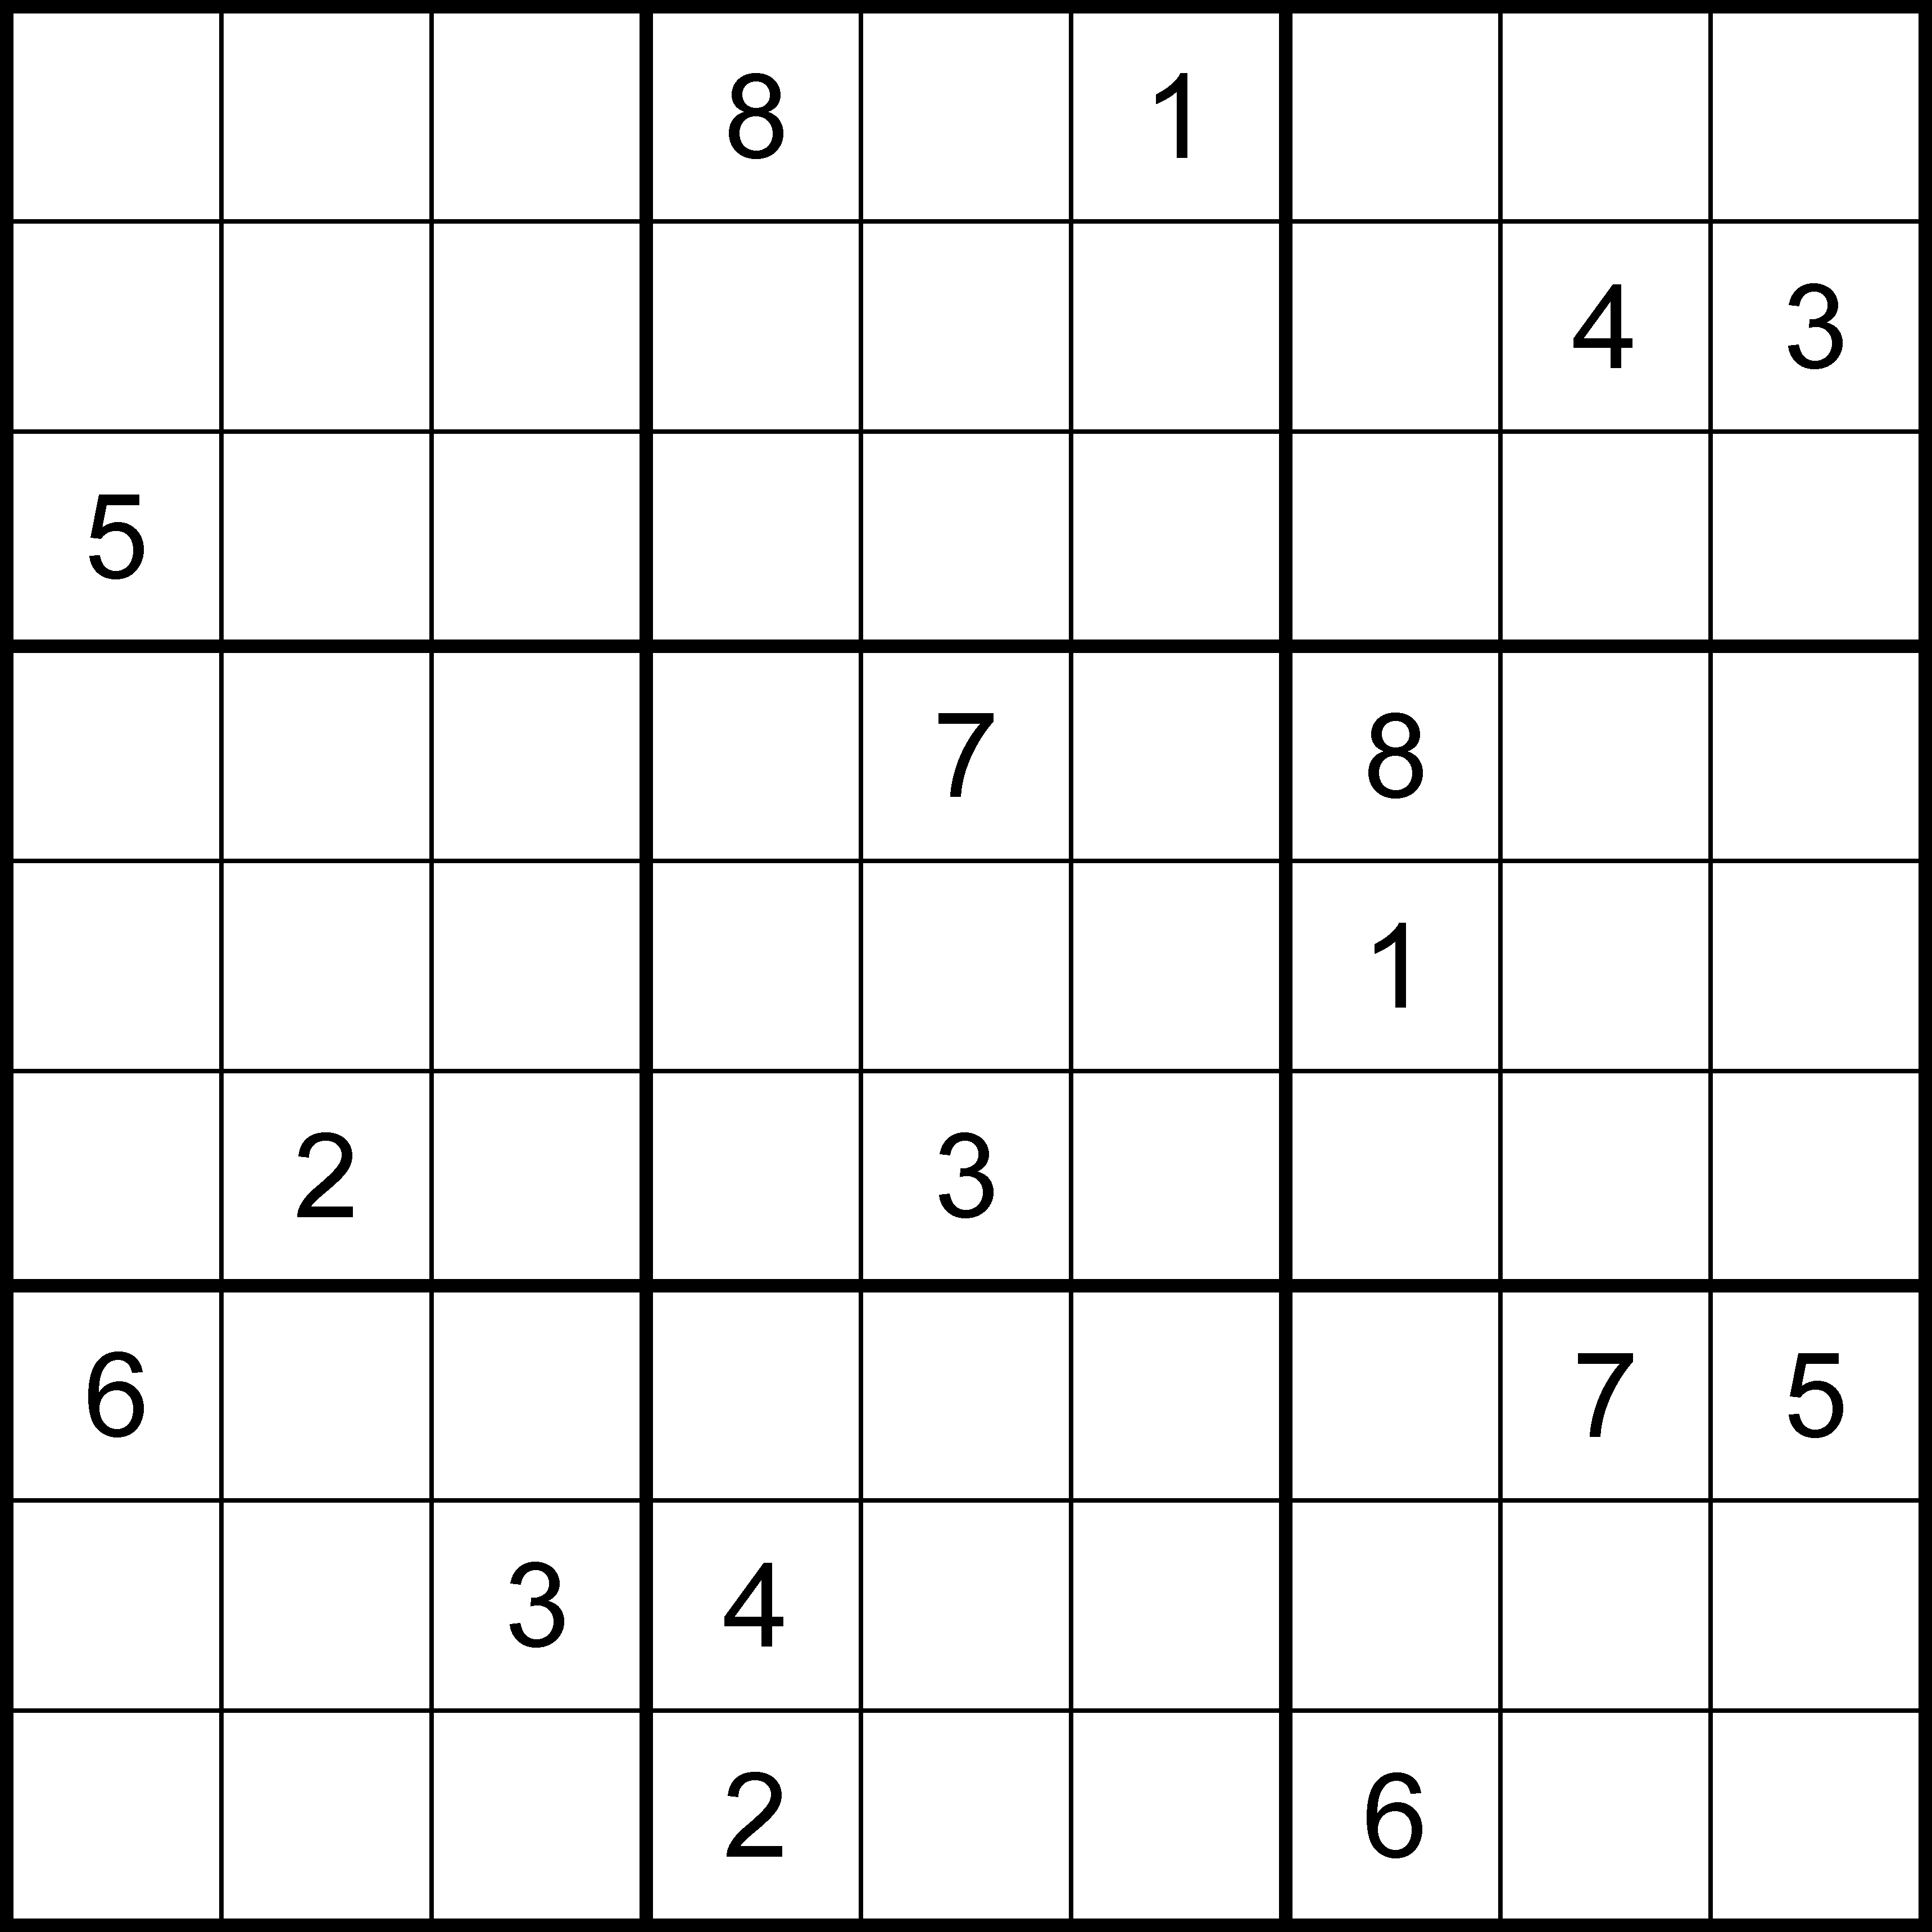
\includegraphics[width=0.5\textwidth]{Figures/17-clue sudoku puzzle (McGuire).png}
\caption{Example of a Sudoku Puzzle with 17 clues by \citet{doi:10.1080/10586458.2013.870056}.}
\label{fig:exampleSudoku}
\end{figure}

\begin{figure}
\centering
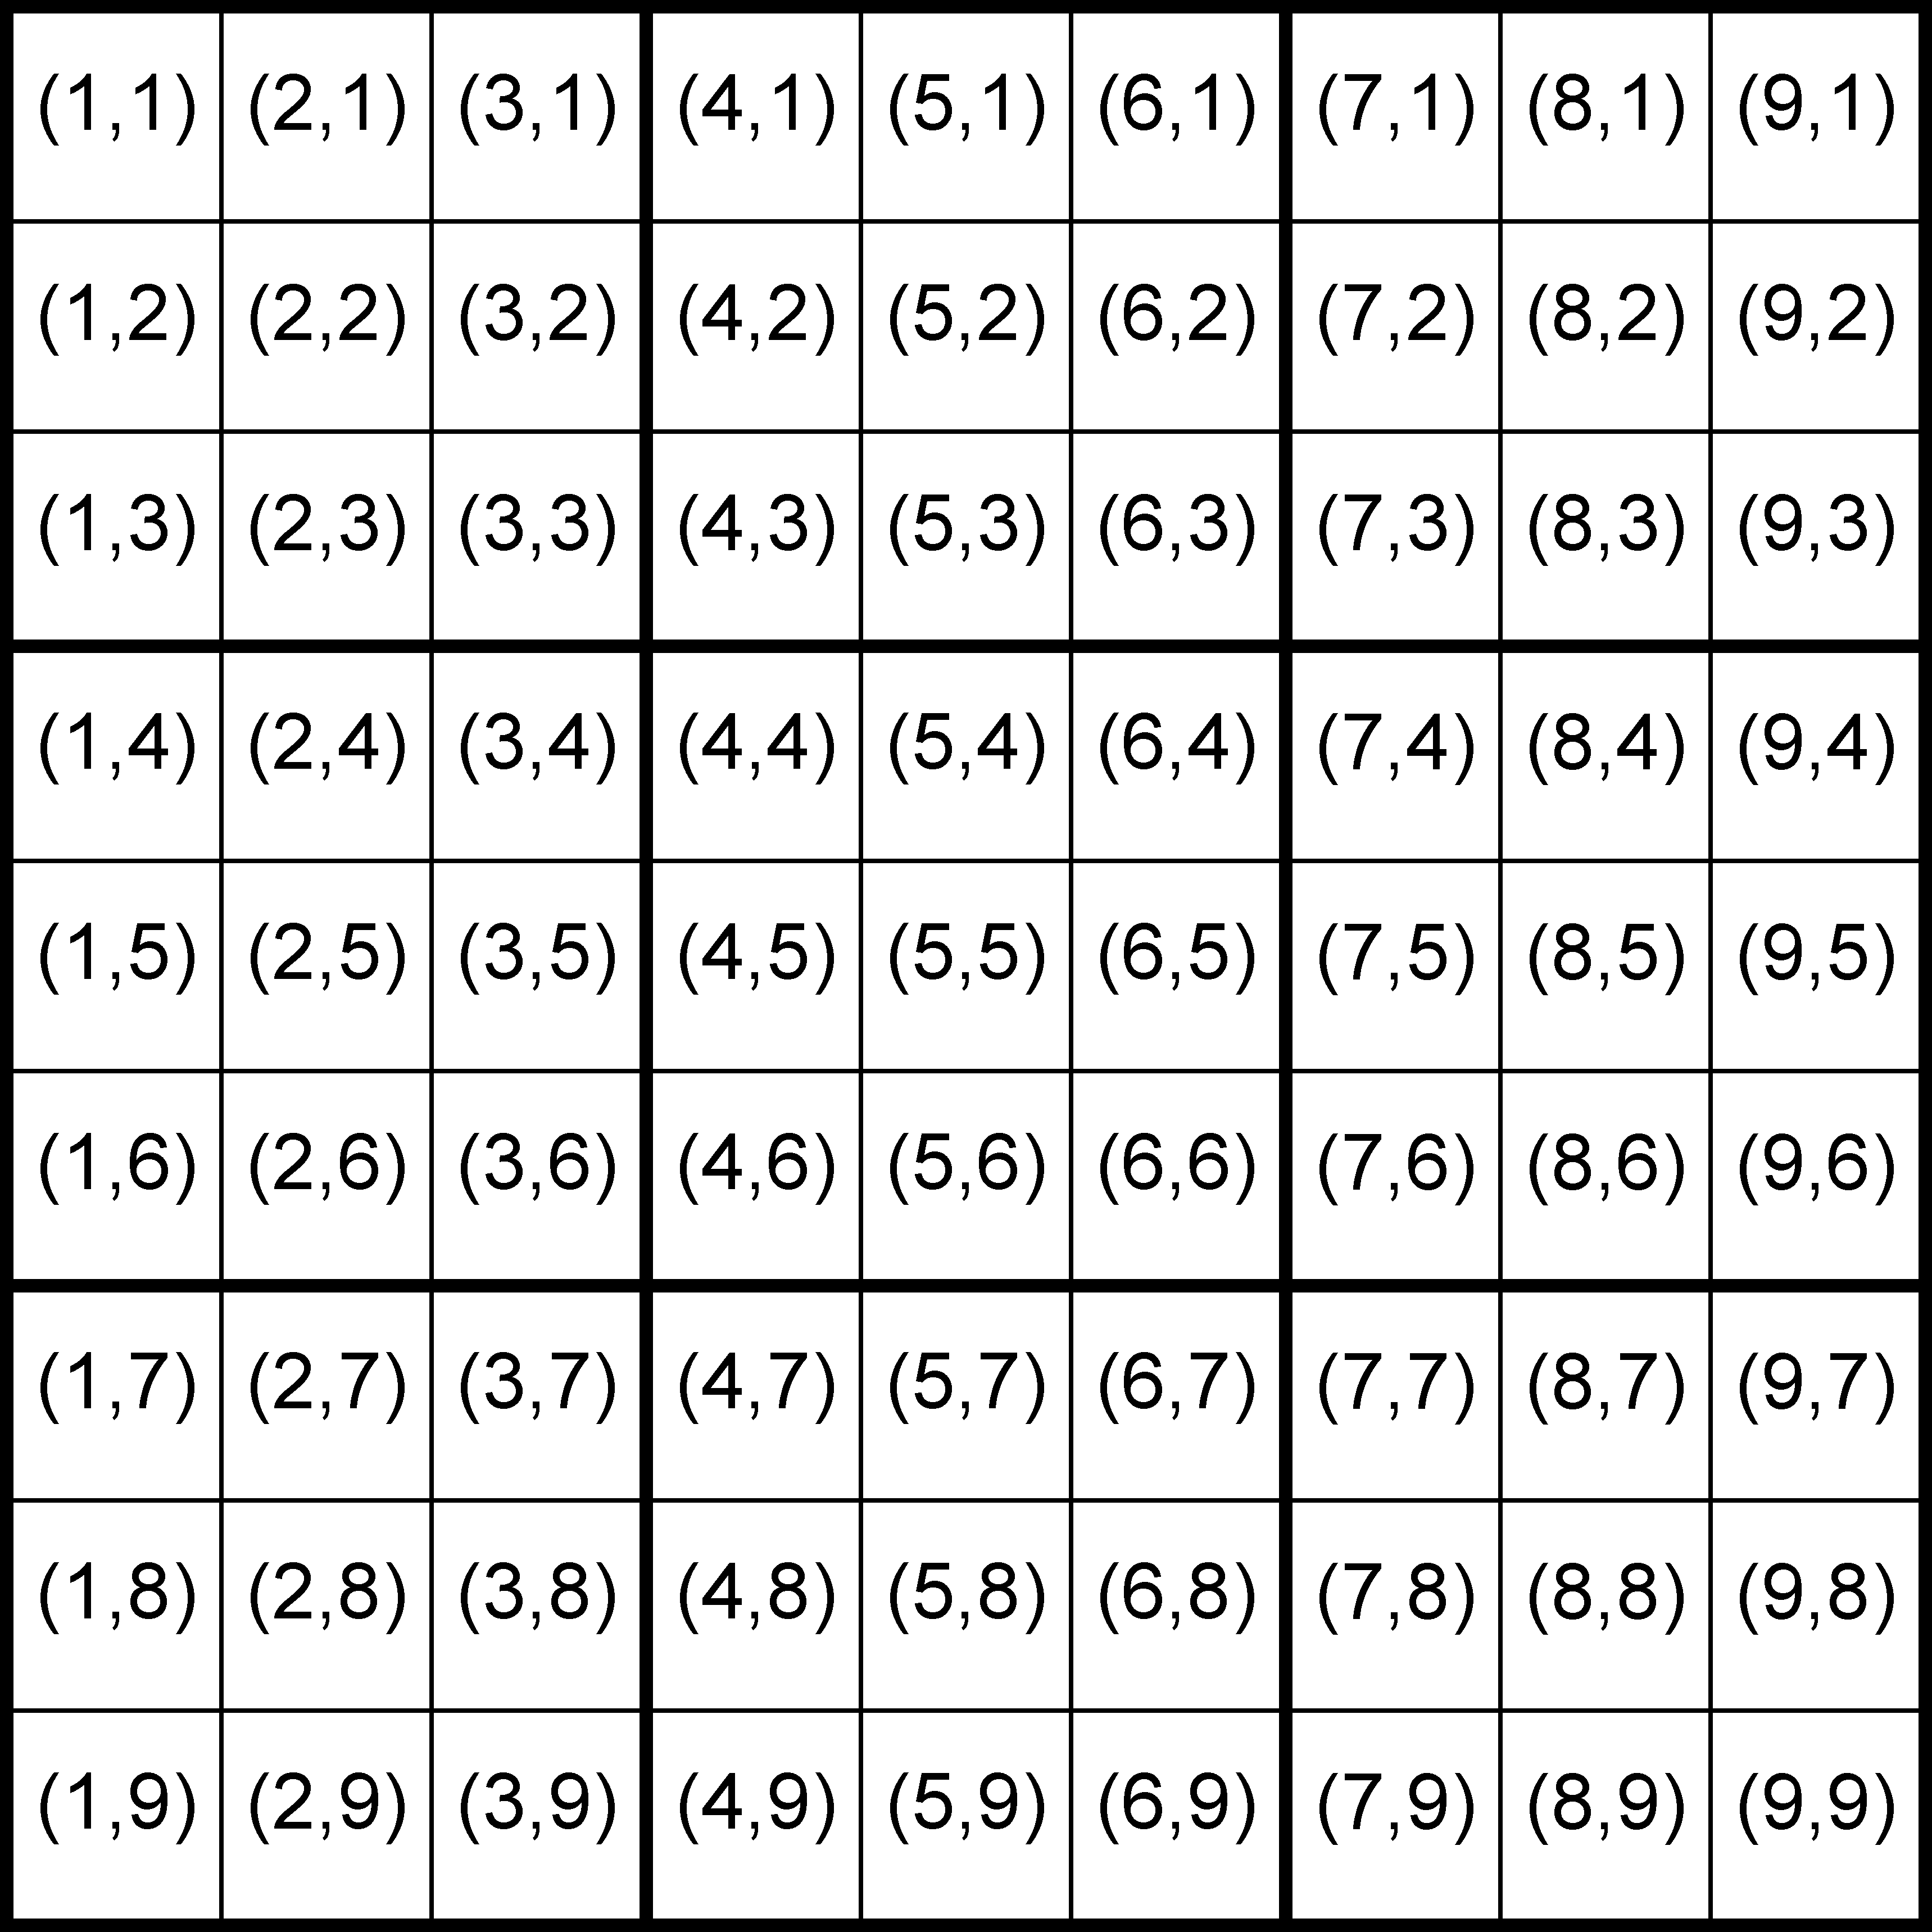
\includegraphics[width=0.5\textwidth]{Figures/GridCoordinates.png}
\caption{Coordinate system for grid cells.}
\label{fig:GridCoordinates}
\end{figure}

